\documentclass[letterpaper,12pt]{article}
\setlength{\headheight}{14.49998pt}
\usepackage{a4wide}
\usepackage{listings}
\usepackage{fancyhdr}
\usepackage{lipsum,graphicx}
\usepackage{bookmark}
\usepackage{amsmath, amsfonts, amssymb, ragged2e}
\usepackage{hyperref} 
\usepackage{times}
\graphicspath{ {C:\Users\10054\OneDrive\luckunately.github.io\CPEN411\Summary\Image} }
\title{Summary of CPEN 411}
\author{Tom Wang}
\date{Fall, 2023}

\fancypagestyle{plain}{
    \fancyhf{}
    \fancyhead[L]{Tom Wang}
    \fancyhead[R]{\thepage}
}

\begin{document}

\maketitle
\thispagestyle{plain}

\section{Terminology}
\subsection{The Iron law}
The sum of each cycle execution time is the total time.

CPI = Cycle per Instruction

\includegraphics*{./Image/The Iron law.png}

\[
    \text{speedup}=\frac{\text{Q1}}{\text{Q2}}
\]

The speedup of Q2 with respect to Q1 is xxx.

\subsection{Amdahl's Law}

\includegraphics*{./Image/Amdahl's Law.png}

\subsection{Dynamic Power}

For CMOS chips, traditional dominant energy consumption has been in switching transistors, called \textbf{dynamic power}.
\[
    \text{Power}_{\text{dynamic}}=0.5*\text{CapacitiveLoad}*\text{Voltage}^2*\text{FrequencySwitched}
\]

For mobile devices, energy might be a better metric:
\[
    \text{Energy}_{\text{dynamic}}=\text{CapacitiveLoad}*\text{Voltage}^2
\]

Capacitive load is a function of the number of transistors connected to output and technology, which determines the capacitance of wires and transistors.

Dropping voltage helps both power and energy.

For a fixed task, slowing the clock rate (frequency switched) reduced power, but not the total energy. However, a slower clock rate might allow lower voltage.

Clock gating: Turn off clocks for the parts that we do not use which saves energy and dynamic power. However, clock skew rises up, it is hard to be precise.

\subsection{Stactic power}

Leakage current flows even when a transistor is off. So there is static power.

\[
    \text{Power}_{\text{static}}=\text{Current}_\text{static}*\text{Voltage}
\]

Leakage of current increases in processors with smaller transistor sizes.

Increasing the number of transistors increases power.

Very slow power systems can gate voltage to inactive modules.

\section{Memory technologies}
\subsection{Learning objectives}
\begin{itemize}
    \item Identify memory technologies used today
    \item Contrast SRAM, RF, CAM, and DRAM structures
    \item Describe the tradeoffs (density, latency, power)
\end{itemize}
\subsection{Memory hirerarchy}
First of all, some definitions:

Storage: SSD or HDD

DRAM: random-access semiconductor memory. Usually consisting of a tiny \textbf{capacitor} and a \textbf{transistor}.
DRAM requires an external memory refresh because of slow leakage on the capacitor.

One trick to not block any code: rewrite a certain portion of it at once, and split it averagely into the refresh cycle. This way DRAM does not block any code for every refresh cycle.

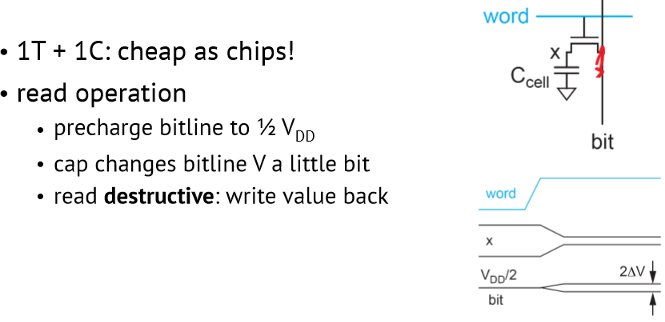
\includegraphics{./Image/DRAM_cells.png}

SRAM: A type of random access memory. Unlike DRAM, it does not need to refresh.
SRAM is commonly used for a computer's cache memory, such as L2 or L3 cache.
SRAM contains 6 transistors in total if counting the transistors to the bit line. Otherwise, 4 transistors.

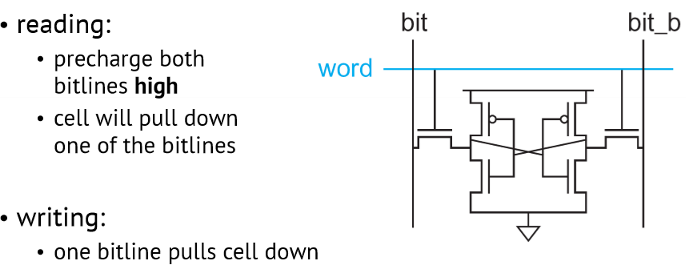
\includegraphics{Image/SRAM_cell.png}

The following is the hierarchy.

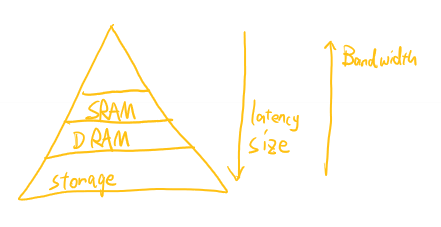
\includegraphics{./Image/Memory_hierarchy.png}

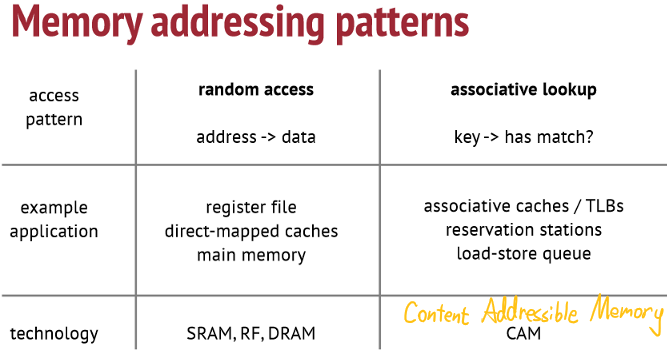
\includegraphics{./Image/Memory_addressing_patterns.png}

\subsection{RAM addressing}

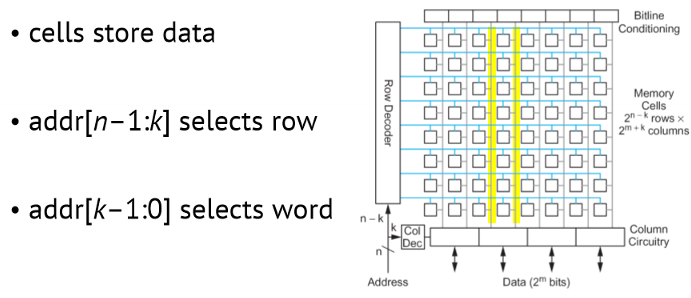
\includegraphics{./Image/RAM_addressing.png}

We turn on the whole row and the whole word to select the address. Here we want `n' to be close to `m'. If n$>>$m, n will dominate latency. Vice versa.

To read, address drives the word line, cells drive the bit lines. Then bit lines are read out and amplified.

To write, address drives the word line. The value drives the bit lines. Then we write the bitline values to the cells. Now cells keep the data.

For DRAM, each bank has a single\-row buffer. It acts as a cache within DRAM.
Row buffer can serve multiple instructions. The first one takes much longer since it needs to fetch from the memory. The rest can directly read from the buffer, much faster.
\begin{itemize}
    \item If an access stream has a locality, a row buffer is kept open. (open policy)
          Row buffer hits are cheap. Row buffer miss is a bank conflict and expensive
          because precharge is on the critical path
    \item If an access stream has little locality, bit lines are precharged
          immediately after access (close-page policy)
          Nearly every access is a row buffer miss. The precharge is usually not on the critical path.
\end{itemize}

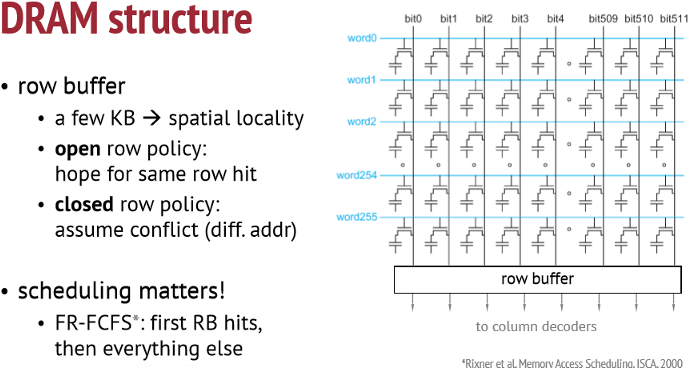
\includegraphics{Image/DRAM_structure.png}

\subsection{Rowhammer}

Repeated same\-row hits in recent DRAMs can flip bits in a neighboring row!

However, you need to access both the upper and lower addresses of the target row. If you only access one of them, then the row buffer will take all the calls due to optimization.

\section{Caches and Prefetching}

\subsection{Avaliable technologies}

\begin{itemize}
    \item DRAM: dense and cheap but slow (10s of ns)
    \item SRAM: about 5 times more area per bit but fast!
          For SRAMs: the smaller the size, the faster the response.
    \item  So now, we have a tradeoff between fast and big.
\end{itemize}

To solve the tradeoff problems, we establish a leveled memory system:

\includegraphics*[scale = 0.8]{./Image/CPU_mem_hierarchy.png}


\subsection{Memory access locality}

\textbf{First some terminology:}

\textbf{Temporal locality}: If the program accesses a single location, then accesses it soon thereafter.

For example, you read the location and write to that location afterward. Y=Y+5

The idea of temporal locality is to keep copies of recently accessed data nearby. (i.e., in small, fast memory)

\includegraphics*{./Image/Exploiting temporal locality.png}

Here we move the data from DRAM into the cache for faster multiple visits.

There are two ways to manage fast storage:
\begin{itemize}
    \item Option 1: scratchpad:
          \begin{itemize}
              \item program copies most useful data. Unlike cache, scratchpad memory is typically not managed by software.
              \item programmer or compiler decides what data or instructions should be placed in the scratchpad
              \item used in GPUs and other contexts
              \item The capacity of scratchpad memory is limited and is typically smaller than the cache memory but larger than CPU registers.
              \item scratchpad memory is usually a single contiguous block of memory, and its size and organization are determined by the programmer.
          \end{itemize}
    \item Option 2: cache
          \begin{itemize}
              \item Managed automatically in hardware where it tracks locality patterns.
              \item Functionally transparent to the programmer(Software).
              \item Cache is organized into multiple levels, typically L1, L2 and sometimes L3.
          \end{itemize}
\end{itemize}

Fully associated cache:
\begin{itemize}
    \item Allows any block of data from the main memory to be placed in any cache location.
    \item There are no restrictions on where a particular block of data can be stored.
    \item There is no set index to determine where to place or find data. We use tags to keep track of which block of data is stored in each cache location:
          \begin{itemize}
              \item Memory block address: to identify which memory block is stored in the cache location
              \item Valid Bit: A valid bit indicates whether the cache location contains valid data. If the valid bit is set, it means that the data in that location is valid and corresponds to the given tag.
              \item Dirty/Modified Bit: To indicate whether the data in the cache location has been modified and needs to be written back to the main memory.
          \end{itemize}
    \item Fully associative caches tend to have fewer cache misses due to conflicts (where multiple memory blocks are complete for the same cache location) because they can accommodate any data block in any cache location.
    \item Implementing a fully associative cache can be more expensive in terms of hardware complexity and cost compared to others. The need for tags and additional logic for managing cache entries adds to the hardware overhead.
    \item Fully associative caches can achieve high hit rates for data access because they can match requested data with any cache entry, regardless of its location within the cache. This makes them particularly effective for applications with irregular memory access patterns.
\end{itemize}

Problems with fully associated caches:

\begin{itemize}
    \item Tag must store the full address of the memory
    \item Address can be in any row, have to search all rows.
\end{itemize}

\textbf{Spatial locality}: After accessing one location, the program accesses a nearby location.

For example, Foreach (var i in Array). accesses all components of the array starting the address of the array.

\includegraphics*{./Image/Spatial locality idea.png}

IDEA: When filling cache entry, also transfer adjacent data.

Memory is divided into blocks (cache lines) with power-of-two size. Blocks start at addresses aligned to block size. Typically 64 bytes for CPU and 128 bytes for GPU.

\includegraphics*{./Image/Memory block illustration.png}

So we include the 8\-byte address in the tag, 64\-byte data in the lower bits of the block. The highest bits are valid and modified bits.

\includegraphics*{./Image/Cache block design.png}

\subsection{Block offset}
Block offset is a component of memory addresses that helps determine the position of a specific byte within a memory block or cache line.

To address individual bytes within a block, the block offset is represented in binary format. The number of bits required for the block offset depends on the block size.
For example, if the block size is 64 bytes, you would need 6 bits to uniquely address any byte within that block.

\[
    \text{Block Offset Bits} =     \text{log}_2(\text{Block Size in Bytes})
\]

\subsection{Direct Mapped cache}

The cache is divided into multiple fixed-size blocks, also known as cache lines.
If there are $2^n$ lines. Then there are $2^m$ partitions in the main memory. Each partition is $2^n$ lines.

A tag has m bit and the index has n bit.

\includegraphics*[scale = 0.55]{./Image/Direct mapped.png}

In a direct-mapped cache, a conflict occurs when multiple memory blocks from the main memory map to the same specific cache slot or line.

\subsection{Set-associative Cache}

IDEA: use cache index to select \textbf{set} of blocks. Each set is like a fully associative cache.

2 way = 2 blocks. 4 way = 4 blocks.

Use the index to search in sets. It is harder to conflict. Needs more data than the \# of ways to conflict.


\subsection{Reuse distance}

\[
    \text{reuse distance} = \text{\# of unique other blocks at this point}
\]

For example, the reuse distance for A at ``ABBCBCCDBBEDBBBA'' is 4 since there are 4 \textbf{unique} blocks before it.

\subsection{Replacement policy}

An algorithm is used to decide which block to evict.

Some ideas for choosing \textbf{replacement victim}
\begin{itemize}
    \item random (Better than you would expect!)
          \begin{itemize}
              \item Select victim uniformly at random
              \item Pros: do not need to remember anything!
          \end{itemize}
    \item least frequently used (LFU)
    \item least recently used (LRU)
          \begin{itemize}
              \item Timestamp per cache block
              \item Mark the ones to `1' when re-referenced. If all get `1', flip them all to `0'.
              \item When choosing one to evict, choose the ones with `0'.
          \end{itemize}
\end{itemize}

\subsection{The 3 Cs (3 types of misses)}

\begin{itemize}
    \item Cold start misses
          \begin{itemize}
              \item first time a block is accessed
              \item increasing size or associativity does not help
              \item can increase the block size
          \end{itemize}
    \item Capacity misses
          \begin{itemize}
              \item access would not be a miss if the cache were infinite
          \end{itemize}
    \item Conflict misses
          \begin{itemize}
              \item set size $<$ number of accesses that map to given set
              \item access would not be a miss if the cache were fully associative
          \end{itemize}
\end{itemize}

\subsection{Cache Performance Impact}

\includegraphics*{./Image/Cache Performance Impact.png}

\subsection{Victim cache}

Victim cache is a small fully associative cache that stores \textbf{recently evicted} lines.
\begin{itemize}
    \item On evict, place in the victim cache
    \item If hit in victim cache, place back to normal cache
    \item Managed similarly to normal cache. E.g., LRU
    \item Adds some extra associativity for some busy lines.
\end{itemize}

\subsection{Types of writes that hit in the cache}

\begin{itemize}
    \item Write-Evict:
          \begin{itemize}
              \item The data is directly written into the memory, then the corresponding cache line would turn the valid bit to 0 so that it could be evicted later.
              \item Might be good for multicore.
          \end{itemize}
    \item Write Through:
          \begin{itemize}
              \item Write the new data into the memory and the corresponding cache line.
              \item Will be good if need multiple visits of the same cache line.
          \end{itemize}
    \item Write back:
          \begin{itemize}
              \item Only writes to the cache, memory only gets the data when evicted from the cache
              \item Since only writing to cache, it is much faster.
              \item However, for multicore, other cores might need to fetch inside a different core's cache to find the right data, which could be even slower.
          \end{itemize}
\end{itemize}

\includegraphics*[scale = 0.8]{./Image/Writes that hits.png}

\subsection{Types of writes that misses in the cache}
\begin{itemize}
    \item Write-allocate:
          \begin{itemize}
              \item The corresponding memory block is loaded into the cache, then we write to the cache. So read then write.
              \item Appropriate when subsequent accesses to the same block are likely (exploits temporal locality)
              \item Can result in unnecessary reads for write operations if the entire block is not going to be used.
          \end{itemize}
    \item Write-no-allocate
          \begin{itemize}
              \item Write is performed directly to the main memory without loading to the cache. So no read.
              \item Reduces cache pollution by avoiding unnecessary reads.
              \item More suitable for write-intensive workloads where reads of recently written data are less likely.
              \item Not able to take advantage of spatial locality
              \item Inefficient use of cache when read is following write
          \end{itemize}
\end{itemize}
\includegraphics*{./Image/Write that miss.png}

\subsection{Evictions in a cache hierarchy}
\begin{itemize}
    \item inclusive
          \begin{itemize}
              \item Lower-level caches contain a superset of the data present in higher-level caches.
              \item E.g., if present in L1, present in L2
              \item Increased storage requirements since stored in multiple cache.
              \item Fetching is simple since only need to check one level.
          \end{itemize}
    \item exclusive
          \begin{itemize}
              \item Each cache level contains a disjoint set of data. No duplicates on different levels.
              \item No redundancy so saves storage.
              \item May result in higher miss rates especially if data frequently migrates between cache levels.
              \item Need to search all cache to find the data.
          \end{itemize}
    \item non-inclusive
          \begin{itemize}
              \item Non-inclusive caches are also known as non-inclusive, non-exclusive or sometimes as set-associative caches.
              \item It is unknown if each level has unique or shared data.
              \item Compromise between storage efficiency and simplicity in coherence management.
          \end{itemize}
\end{itemize}

\includegraphics*[scale = 0.9]{./Image/Eviction in a cache hierarchy.png}

\subsection{Read and Write}
When do you cause memory to write?

load: reading data from memory

store: writing data to memory

When you load and there is a dirty/modified line, then you write that line to the memory and then load it.

When you store, we evict a cache line which can welcome a memory read.

\subsection{L1 Separating instruction and data}

\includegraphics*{./Image/Instruction and Data separation.png}

We separate instruction and data in L1 because:
\begin{itemize}
    \item Reduce latency in instructions so that there are no instruction load stalls.
          \begin{itemize}
              \item Instruction stall, also known as pipeline stall or pipeline bubble.
              \item Wastes CPU cycles.
              \item Instruction pipelines are designed to process multiple instructions simultaneously by breaking down the instruction execution into stages (fetch, decode, execute, etc.). Stalls disrupt the smooth flow of instructions through these stages, leading to a reduction in the overall instruction throughput. This directly impacts the performance of the processor.
          \end{itemize}
    \item Avoid friendly fire: if together, data accesses might evict the program's instructions.
\end{itemize}

\subsection{Lookup-free cache. MSHR}
MSHR = Miss Status Handling Register.

MSHR is a data structure or a set of registers within a cache controller that keeps track of the status of cache misses. When a processor issues a load or store instruction and encounters a cache miss, the MSHR helps manage the process of fetching the missing data from the next level of the memory hierarchy (usually main memory) and updating the cache.

\begin{itemize}
    \item MSHR keeps track of the cache misses that are currently in progress. Each entry in the MSHR corresponds to a pending cache miss. This allows the cache controller to manage multiple concurrent misses effectively
    \item MSHR stores information about the memory address that caused the cache miss. This information is used to identify and match incoming data when it returns from main memory.
    \item MSHR also holds a \textit{Data Buffering} to store the incoming data associated with a cache miss. It holds the data till it can be written to the cache.
    \item This way, it groups all data going to 1 line and sends only 1 request.
\end{itemize}

\subsection{Prefetching}

Prefetching is a technique used in computer systems to improve memory access performance by fetching data into a cache or main memory before it is actually needed by the processor. The goal of prefetching is to reduce the latency associated with memory access, especially in situations where the processor is likely to encounter cache misses.

\begin{itemize}
    \item Use patterns usually to observe the next memory access
    \item Hardware Prefetching: Modern processors often have dedicated hardware units that analyze memory access patterns and automatically issue prefetch requests to fetch data into the cache.
    \item Software Prefetching: programmers or compilers can also insert prefetch instructions or hints in the code to suggest which data should be prefetched. However, this requires a good understanding of the program's memory access patterns.
    \item Sequential Prefetching: Predict that the processor will access contiguous memory locations. Effective for loops or linear data access patterns.
          \begin{itemize}
              \item Stream buffer: buffer sequential access stream. maybe several buffers for multiple streams.
              \item if hit in stream buffer, move the whole buffer to cache.
              \item However, if the next fetch jumps, then it does not work.
          \end{itemize}
    \item Stride Prefetching: Predict the stride (the constant difference between consecutive memory addresses) and prefetching data at regular intervals. Beneficial for non-contiguous but predictable memory access patterns.
          \begin{itemize}
              \item Track previous address, stride, correctness.
              \item if predictions confirmed, keep prefetching:
              \item An FSM approach:

                    \includegraphics*{./Image/Stride FSM.png}

              \item An example flow chart:
              \item \includegraphics*{./Image/Stride example.png}
          \end{itemize}
    \item Stream Prefetching: Similar but more adaptive to Stride. It dynamically adjusts the prefetch distance based on the observed memory access behavior.
    \item Prefetching pros and cons:
          \begin{itemize}
              \item Reduced memory latency.
              \item Improve memory subsystem throughput, allowing the processor to continue executing instructions without waiting for memory accesses.
              \item Enhance cache utilization: Prefetching helps make more efficient use of the cache space by populating it with data that is likely to be accessed soon.
              \item However not always Beneficial, incorrect prefetching decisions can lead to wasted bandwidth and can cause pollution. If the miss rate is too high, the CPU will turn the predictor off.
          \end{itemize}
\end{itemize}


\section*{Improve Cache Articles:}

1. Adaptive Insertion Policies for High-Performance Caching  ISCA 2007: This is present in older CPUs:\url{https://dl.acm.org/doi/10.1145/1250662.1250709}

2. Tree-Based P-LRU (pseudo-LRU) Replacement Policy: This is present in older embedded CPUs.
Please read Chapter 3, Section 4 of this
\hyperlink{https://citeseerx.ist.psu.edu/viewdoc/download?doi=10.1.1.217.3594&rep=rep1&type=pdf}{document}
from ARM.

The Wikipedia page gives you a high-level overview:

\url{https://en.wikipedia.org/wiki/Pseudo-LRU}

3. SRRiP and DRRiP Policies  ISCA 2010: This is present in modern CPUs --> \url{https://dl.acm.org/doi/10.1145/1815961.1815971}

4. Signature-based hit prediction  MICRO 2011: This is an academic work --> \url{https://dl.acm.org/doi/10.1145/2155620.2155671}

\begin{itemize}
    \item Victim selection policy: Decides which line gets evicted for storing an incoming line.
    \item Insertion policy: Decides where in the replacement list the incoming line is placed.
\end{itemize}

\begin{enumerate}
    \item LRU: Least recently used.
          In an LRU cache, data is stored in a limited-sized cache memory, which can hold a fixed number of items.

          Each time an item is accessed or used, it is marked as the most recently used item. This timestamp or marker is typically recorded in a data structure like a linked list or an ordered array.

          When the cache reaches its capacity limit and a new item needs to be added, the LRU algorithm identifies and evicts the least recently used item from the cache.

          LRU is designed to optimize cache usage for scenarios where some items are accessed much more frequently than others.

          One notable drawback is that it requires maintaining a record of the access order, which can be memory-intensive.

          Also, it might not be good when access patterns change suddenly or there are hot items that are very frequently accessed, which can cause frequent cache evictions.

    \item LIP: LRU Insertion policy.
          Instead of placing all incoming lines into MRU(Most recently used), they are all put into LRU and only prompted to MRU if they get referenced while in the LRU position.

          LIP prevents thrashing for workloads that reuse a working set greater than the available cache size.

          However, LIP may retain the lines in the non-LRU position of the recency stack even if they cease to be re-referenced. Since LIP does not have an aging mechanism, it may not respond to changes in the working set of the given application.

    \item BIP: Bimodal Insertion Policy.
          Similar to LIP except that it infrequently (with a low probability) places some incoming lines into the MRU position.

          BIP is regulated by a parameter, bimodal throttle parameter $\epsilon$, which controls the percentage of incoming lines that are placed in the MRU position.

          Both LRU and LIP can be seen as a special case of BIP with $\epsilon = 1,0$ respectively.

    \item Dynamic Insertion Policy BIP(DIP)
          Dynamically estimates the number of misses incurred by the two competing insertion policies (BIP and LRU). Select the policy that incurs the fewest misses.

          The simplest way is to implement LRU and BIP in two extra tag directories and keep track of which of the two policies is doing better. The main target directory of the cache can then use the policy that incurs the fewest misses.

          The figure below demonstrates the working of DIP. Let MTD be the main tag directory of the cache, The two competing policies LRU and BIP are each implemented in a separate Auxiliary Tag Directory (ATD). Both ATD-LRU and ATD-BIP have the same associativity as the MTD. The access stream visible to MTD is also applied to both of them. A saturating counter, which we call \textit{Policy Selector} (PSEL), keeps track of which of the two incurs a few misses. All operations on PSEL are done using saturating arithmetic. A miss in LRU increments PSEL and a miss in BIP decrements PSEL. The most significant Bit (MSB) of OSEL is an indicator of which of the two policies incurs fewer misses. If MSB od PSEL is 1, MTD uses BIP, otherwise LRU.

          \includegraphics*[scale=0.7]{./Image/DIP.png}

          However, it does require two more ATDs which can be troublesome. So instead, we introduce \textbf{Set Dueling:}

          Set Dueling dedicates a few sets of the cache to each of the two competing policies. The reset sets are follower sets that use a policy that incurs fewer misses on the dedicated sets.

          This kind of DIP is called \textit{DIP-SD}

          \includegraphics*[scale=0.7]{./Image/DIP-SD.png}

          A miss in LRU sets increments PSEL whereas a miss in BIP decrements PSEL. If the MSB of PSEL is 0, the follower sets use the LRU policy. Otherwise, the follower uses BIP.
\end{enumerate}

\section{Virtual Memory}

A brief intro to why virtual memory:

Problem: The operating system needs to multitask (time-multiplex)
\begin{itemize}
    \item But all programs assume address space starts at 0
    \item Enough physical RAM to run one program but not enough to fit all of them at once.
\end{itemize}

Solution: separate address space per program
\begin{itemize}
    \item Each program has a separate address space ID (ASID)
    \item Program executes using virtual addresses (VA) so that the program thinks it has all of the memory.
    \item CPU and OS translate to physical address (PA)
    \item Same VA with different ASID would map to a different physical address.
\end{itemize}

\subsection{Paged virtual memory}

\includegraphics*{./Image/paged virtual memory.png}

Divide the address into pages. Map used ones into a physical address in memory. Leave the rest in Disk.

The physical address is translated from VA by OS. Offset is the byte address of a byte in a page. So size of page can be determined as $2^{\text{offset bit}}$

\includegraphics*{./Image/Page table register.png}

Page table register is used to map. The valid bit in it indicates if it is on the disk or in the memory. if (valid == 0) on disk.

The address of the virtual page number in the page table register holds the physical address.

The size of the table depends on the bit number of the virtual page number since the page table should cover all of the virtual pages.

For example, for a n-bit virtual address and m-bit page offset, the virtual page number is (n-m) bit. So the number of entries for the table is $2^{n-m}$

For programs that use virtual memory, address translation is required for every data mem access and every instruction fetch since it does not have the actual address of data.

\subsection{Efficiency of page table}

Where to put the page table?
\begin{itemize}
    \item Option 1: on-chip near the CPU (like the L1 Cache)
          \begin{itemize}
              \item pros: very fast access
              \item cons: 1 M entries size $>>$ any reasonable L1 cache
          \end{itemize}
    \item Option 2: off-chip in main memory
          \begin{itemize}
              \item pros: size might not be a problem.
              \item cons: access is very slow (We need 2 access for each instruction)
              \item cons: per-process tables still have lots of memory.
          \end{itemize}
\end{itemize}

Observations in real programs:
\begin{itemize}
    \item Each process needs its own page table. 100s-1000s processes could easily be active.
    \item Page tables are sparse: few programs use the entire address space.
\end{itemize}

Solution: Multi-level page tables (a.k.a hierarchical page tables). Instead of using a single, flat table to map virtual addresses to physical addresses, a multi-level page table divides the task into multiple levels of tables, forming a hierarchy.

\begin{itemize}
    \item Depending on the number of levels, higher-order bits are used as an index in the first-level page table.
    \item The entry in the first-level page table points to the second-level page table.
    \item The lower-order bits are used as an index in the second-level page table, which contains the final page frame information.
\end{itemize}

Benefits:
\begin{itemize}
    \item Space Efficiency: reduce the amount of memory needed for the page table, especially when dealing with sparse address spaces where not all address space is in use.
    \item Flexibility: Different levels of the page table hierarchy can have varying sizes, allowing for flexibility in optimizing memory usage.
\end{itemize}

\includegraphics*[scale = 0.8]{./Image/Multi-level PT.png}

\subsection{Translation-related exceptions}

\begin{itemize}
    \item Page faults:
          \begin{itemize}
              \item page is accessible, but it is sitting on disk. It happens all the time!
              \item This is not a program error!
              \item resume instruction execution once a page in RAM.
          \end{itemize}
    \item Segmentation fault/ general protection fault
          \begin{itemize}
              \item page is not user-accessible
              \item page is R/O (read-only) but it tries to write/execute.
              \item program terminated (unless caught)
              \item Meltdown avoided this by mis-speculating.
          \end{itemize}
\end{itemize}

\subsection{Translation Lookaside Buffer (TLB)}

VA to PA translation is needed for every memory access. Lookup in big multi-level page tables is really slow.

We use TLB, which is a small cache for the most frequently used virtual page number (VPN) to physical page number (PPN) lookups.

\begin{itemize}
    \item If hit, saves a lot of cycles.
    \item If miss, engage page table walker to look for it.
\end{itemize}

Upon page fault, we evict the old page and bring in the new page. When switching to a different program, we need to flush TLB since it is in a different virtual address space.

\subsection{Types of address translation}
\includegraphics*{./Image/Types of address translation.png}
\begin{itemize}
    \item Physically addressed cache:
          If hit in TLB, directly translate VA into PA and access it. Else, look into PTE mem.
    \item Virtually addressed cache:
          The cache only contains the VA of one program. Then we can go from the cache if miss then TLB then mem. Otherwise PTE.
    \item Overlap is obviously the fastest. But the structure needs some special arrangement.
\end{itemize}

Increasing the size of the L1 cache would also increase the misses due to flushing VA L1 caches:

\includegraphics*[scale = 0.7]{./Image/VA cache miss.png}

\subsection{Overlapping TLB and L1 cache accesses}

\includegraphics*[scale = 0.7]{./Image/Overlapping TLB and L1 cache accesses.png}

Example problem:

Suppose pages are 4KB. D cache is a 2-way set-associative maximum cache size?

Page = 4kb = $2^{12}\implies$ set = 6bit = $2^6$ and byte = 6 bit = $2^6$.

Set associativity is 2: size = $set\times associativity \times byte=2^6\times 2\times 2^6=2^{13}=8$KB.

\subsection{VA to PA and synonym problem}

Problem: some address bits change when mapping VA to PA because the page is larger than the page offset compacity. For example, the index of 7 bits is the offset of 6 bits but your page offset is 12 bits only.
Possible solutions:
\begin{itemize}
    \item bigger page sizes. (Increase the page offset to be 13)
    \item more associativity. (Allow a 2\-way associativity)
    \item Make sure the VA keeps the extra index bit the same as before. So maybe there is only half of VA that it is allowed to get in. (Hard to do when there are more bits needed to keep the same)
\end{itemize}

Synonym problem example:

We have a 64KB direct-mapped cache and 16-byte blocks.

\begin{itemize}
    \item total length is 16 since $2^{16}$bit=64KB
    \item block offset is 4bits, so addr[3:0]
    \item The reset is cache index, addr[15:4]
\end{itemize}

If we only have a 4KB page, then each address of the page corresponds to $\frac{64}{4}=16$ other cache.
So 16 synonym locations for every physical address.

\section{Pipelines}

Let's look at a simple pipelining structure.

\includegraphics*[scale = 0.7]{./Image/Simple pipeline.png}

Each stage is a pipeline register. We do one thing at one stage.

However, flip-flops have latency. So we cannot divide too many stages since the charging latency of flip-flop limits it.

Ideal pipeline:
\begin{itemize}
    \item Uniform sub-computations: each stage has the same delay, achieved by balancing pipeline stages.
    \item Identical computations: each computation uses the same number of stages.
    \item Independent computations: start a new computation each cycle.
\end{itemize}

\subsection{Dependency}

A problematic pipeline:

\includegraphics*[scale = 0.7]{./Image/Problematic pipeline.png}

If we are supposed to read the written R1 before decoding it, then the R1 value read before it is a ``stale value''.

So reading the value depends on the previous instructions. Need to make sure you can access the meaningful value after the previous instruction stores it.

\includegraphics*[scale = 0.7]{./Image/pipeline control signal.png}

We use the signals that go along with the instructions. The signal can stall the pipeline so that we can make sure the value is meaningful.

\subsection{Hazards}

\includegraphics*[scale = 0.7]{./Image/Pipeline Hazards.png}

\begin{itemize}
    \item R1 is the destination of the ADD instruction.
    \item R1 is also the source of the rest of the instructions.
    \item R1 introduces dependencies which causes \textbf{Hazards}
    \item In \textbf{Cycle 3 and 4}, we need the value of R1, but R1 is updated in \textbf{Cycle 5}!
    \item Everything at or after cycle 5 is ok.
\end{itemize}

There are three types of hazards
\begin{itemize}
    \item Structural Hazards
    \item Data Hazards
    \item Control Hazards
\end{itemize}
\subsubsection{Structural Hazards}
Caused by resource conflicts:
\begin{itemize}
    \item Two or more instructions want to use the same hardware at the same time.
    \item E.g., fetch the instruction and write to memory at the same time, but you can execute one instruction at a time.
    \item One solution is to stall it and wait for the earlier instruction to finish using the resource.
    \item The other solution is to add more hardware so that multiple instructions can be executed at the same time.
\end{itemize}

Example:
\includegraphics*[scale = 0.7]{./Image/Structural Hazard example.png}

So in this example, both instructions want to access the memory at the same time. The solution is to stall the later instructions.

\includegraphics*[scale = 0.7]{./Image/Structural Hazard solution.png}

\subsubsection{Data Hazards}

\begin{enumerate}
    \item Read after write (RAW) hazards:
          Note the data dependencies of the following instructions:

          \includegraphics*[scale = 0.7]{./Image/RAW instructions.png}

          The solution to it is \textbf{Forwarding}: Sending the data to the next execute stage as it is in CPU before writing back.

          \includegraphics*[scale = 0.8]{./Image/Forwarding.png}

          By adding a mux for all the next stages it is possible for it to forward the data into the next instruction ALU. These muxes are called \textbf{Forwarding Mux}

    \item Write after write (WAW) hazards:

          An example is ``ADD R1, R2, R3'' then ``SUB R1, R2, R4''.

          For this case, we can simply ignore the first line since it will be overwritten anyway, which does not cause any problems.
    \item Write after read (WAR) hazards:

          An example is ``ADD R1, R2, R3'' then ``SUB R2, R4, R5''.

          Just use a temporary register to keep the value you need to write to R2 or change to a different register selected by the CPU. Not a big deal.
\end{enumerate}

\subsubsection{Control Hazards}

Control Hazards are due to branches. The branch may or may not change program counters (PC). So which instruction should follow a branch depends upon the result of executing the branch instructions.

The pipeline can only choose one branch to continue. If not correct, then the execution is wasted.

\begin{itemize}
    \item Option 1 is to stall it. Wait for you to know the branch value before continuing.
    \item Option 2 does branch prediction:
          Branches tend to be ``weakly biased'' meaning that they are taken and not taken roughly the same number of times. So half of the time, we might be right! So now we need a way to correct the behavior if predicted wrong.

          If correct, we know by the end of the branch instruction, and we are happy, so nothing we need to do.

          If not correct, at the next cycle, we need to fix all the incorrect predictions. Squash incorrectly fetched instructions (discard) and start fetching correct instructions.

    \item Option 3 is to delay branches:

          Here is some compiler optimization that can be done.

          Place useful instructions after branch instructions if possible.

          \begin{itemize}
              \item Put instructions that are before the branch that the branch is \textbf{not dependent} on. And it should always improve the performance.
              \item If from branch target: Must be OK to execute if the branch is not taken and improves the performance if it is taken.
              \item If from fall through: Must be OK to execute if the branch is taken and improves the performance if it is not taken.
          \end{itemize}
\end{itemize}


\subsection{Dependencies}
Define dependency: Two instructions use the same register or memory location but no data passes between them. Dependency is on data location (name), not value (contents at location).

\begin{enumerate}
    \item True dependency and RAW hazards:
          A true dependency leads to a `RAW' hazard if the hardware can perform the read before the write.

          \includegraphics*{./Image/true dependency example.png}

    \item Anti-dependencies and WAR hazards:

          \includegraphics*{./Image/Anti-dependency example.png}

          Instructions I and J cannot be reordered, otherwise value will be changed.

          So anti-dependency reuses the names. If anti-dependency causes a hazard in the pipeline, it is called a WAR hazard.

    \item Output dependency and WAW hazards:

          \includegraphics*{./Image/output dependency example.png}

          Instructions I and J cannot be reordered, otherwise value will be changed.

          So it also resolves from the reuse of the name. If an output dependency causes a hazard in the pipeline, it is a WAW hazard.
\end{enumerate}

\subsection{Pipelined function units}

So the ALU or the execution unit might not always be the same length.

\includegraphics*[scale = 0.5]{./Image/ALU differnt length.png}

So it brings up more challenges:
\begin{itemize}
    \item Longer RAW hazards. (Might need to wait for longer so that you can read the executed value)
    \item Structural hazard for MEM, WB. (might have multiple requests to access them at the same time.)
\end{itemize}

\subsubsection{Scoreboard: tracking register accesses}

\includegraphics*{./Image/Score board.png}

For each reg, track ``will be written to by in-flight instruction'' info.

\begin{itemize}
    \item \textbf{Set bit} for destination register at end of \textbf{decode}.
    \item \textbf{clear bit} when instruction \textbf{reaches writeback}.
\end{itemize}

So if new instruction \textbf{reads or will write} a register with the bit set, stall in the decode stage.

So for a ``in-order'' scoreboard execution:
\begin{itemize}
    \item scoreboard: a bit-array, 1-bit for each GPR(General Purpose Register)
          if the bit is not set: the register has valid data. If set: the register has stale data. Some in-flight instruction will write them.
    \item issue in\-order:
          For example: (SB stands for scoreboard)

          RD $\leftarrow$ Fn(RS, RT) // An operation that reads RS and RT and writes RD somehow.
          \begin{itemize}
              \item if (RS.SB()$||$RT.SB()) RAW.stall(); // stall if either RS or RT has stale data
              \item else if (RD.SB()) WAW.stall(); // stall if RD has stale data
              \item else, dispatch to function Fn and set RD.SB to 1;
          \end{itemize}
\end{itemize}

After completion out-of-order: Update GPR[RD], clear RD.SB();

\subsection{Register Renaming}

Note that WAW and WAR come from name dependency which can be solved if there are infinite supply of names.

\subsection{Tomasulo algorithm}

\subsubsection{Hardware}

There is a reservation station in front of each functional unit(FU). FU is a buffer that stores instructions waiting for operands.

\begin{itemize}
    \item Registers in instructions renamed to tags.
    \item Destination register gets fresh tag: mapping to reg. alias table (RAT)
    \item Source register gets corresponding tags from RAT
    \item Track data dependencies directly: no WAW or WAR hazards
\end{itemize}

Results broadcast on \textbf{common data bus} (CDB). Each result carries the tag of source RS when it is produced. All register stations (RS) and register files (RF) listen to the CDB for tages they want values for and pick up corresponding values on CDB.

\subsubsection{Stages}

\begin{itemize}
    \item issue
          \begin{itemize}
              \item If have a free RS (no structural hazard), allocate RS entry
              \item lookup source operand registers in RF: get either values or tags. (Get value if available, otherwise, need tags since waiting for value)
              \item Rename destination register to allocated RS entry tag.
          \end{itemize}
    \item execute
          \begin{itemize}
              \item Listen for unready operand tags on the CDB, pickup values.
              \item Once all operands are ready, commence execution.
          \end{itemize}
    \item write result
          \begin{itemize}
              \item Broadcast $<$dst tag, result$>$ on the CDB
              \item Interested RSs and RF will see the tag and update the value
              \item Mark reservation station available
          \end{itemize}
\end{itemize}


\section{In-order commit and multiple issue}

The problem arises from the difference between completion and commitment:
\begin{itemize}
    \item Complete: Executing unit has finished executing the instruction
    \item Commit: Update the value in the register file
\end{itemize}

So if we design our CPU that commits and completes at the same time as how simple Tomasulo algorithm states, RF will be updated at the same time as completion. However, might need to discard some values if we found some exceptions in completion. This means there might be some that we should not update into the RF.

\subsection{Why would we flush the pipeline? Exceptions!}
\begin{itemize}
    \item Mispredicted branch
    \item External interrupt (key press)
    \item Program fault (div. by 0, segfault)
    \item Trap (debugger breakpoint)
    \item OS context switch (timer)
    \item Page fault (unmapped virtual address)
\end{itemize}

All above are called exceptions. For each exception that we detected at \textbf{execution time,} it requires \textbf{transfer of control} to an OS interrupt service routine. Then we may need to \textbf{resume the original program} as if nothing happened.

\subsubsection{Precise exceptions}

If an architectural state is updated by \textbf{all instructions before faulting instruction} and \textbf{none} after (and including) faulting instruction, then the pipeline supports \textbf{precise exceptions}. Note that not all architectures do.

\includegraphics*{Image/precise exception.jpg}

\subsubsection{Exceptions in an in-order pipeline}
When exception strikes:
\begin{enumerate}
    \item switch instruction fetch to \textbf{exception handler}
    \item convert instructions after and including ``faulting instruction'' to \textbf{nops} (e.g., turn off write enable control bits)
    \item \textbf{remember PC} (program counter) of faulting instruction
\end{enumerate}

\subsection{Dealing with exceptions without stalling}

\subsubsection{Speculative Execution}

The goal of speculative execution is to support the exception of instructions fetched following a branch prediction \underbar{before} we know if the prediction is correct.

However, the problem is that instructions after the branch should not update the register file before confirming that the branch is correct. Make sure the control/branch hazard is resolved before proceeding.

Speculative execution describes the capacity of the way to \textbf{cancel mispredicted path}.

\subsubsection{Completion and commit}
\begin{itemize}
    \item Insight: the problem arises in writing to RF, not finishing the computation early.
    \item Idea: compute and buffer the result but \textbf{delay the RF write} until prior instructions \underbar{guaranteed} to retire (not speculative, no exceptions)
\end{itemize}

Now we can split writeback into \textbf{completion and commit}.
\begin{itemize}
    \item Completion = buffer computed result
    \item Commit = write result to RF
\end{itemize}

\subsubsection{The recorder Buffer (ROB)}

ROB is a process between completion and commit:

\includegraphics*[scale = 0.7]{Image/ROB figure.jpg}

\begin{itemize}
    \item stores instructions in \textbf{program order} (a FIFO)
    \item \textbf{buffers} computed results before RF write
    \item commits in \textbf{program order}
\end{itemize}

ROB tracks the execution status for each instruction

\includegraphics*[scale=0.9]{Image/ROB execution stage.jpg}

Depending on if there is a branch it is waiting for, the issue stage allocates RS and ROB entry may or may not:
\begin{itemize}
    \item use ROB entry to hold computed value
    \item use ROB entry ID as renaming tag
\end{itemize}

\subsection{Superscalar execution}

Pipeline CPI = Ideal CPI + Structural stalls + Data hazard stalls + Control hazard stalls.

We know how to remove/reduce stalls: pipelining, forwarding, out-of-order execution, speculative execution\ldots

So we also want to reduce the ideal CPI:
\begin{itemize}
    \item ideal CPI limited by issue rate: 1 instruction per cycle.
    \item What if we allow more instructions to be executed per cycle?
\end{itemize}

\subsubsection{Stactically Scheduled Superscalar}
Issue up to N instructions per cycle. At issue:
\begin{itemize}
    \item check each instruction for hazards with co-issued instructions that are \textbf{earlier in program order}
    \item also against all earlier \textbf{instrctions still in execution}
\end{itemize}
\includegraphics*{Image/Stactically Scheduled Superscalar.jpg}

above: comparisons to avoid RAW, WAR, and WAW hazards in a 3-wide in-order superscalar.

Red and blue checks for WAW and WAR. Green checks for RAW.

\subsubsection{2-Issue In-order Superscalar}
\includegraphics*{Image/2-Issue In-order Superscalar.jpg}

So here we have a pipeline for Integer and FP. There are multiple issues with Dynamic Scheduling:
\begin{itemize}
    \item needs an extension of Tomasulo's algorithm
    \item key challenge: renames, assign RS, and update pipeline control tables for \textbf{for multiple instrcstions}
\end{itemize}
We can either run this at a higher clock speed or add logic to rename multiple instructions at once.

\includegraphics*[scale=0.8]{Image/Tomasulo with too wide issue.jpg}

So here, we have two CDBs that can handle two outputs at once. Then we run the load buffer at two times the speed or two assigning per cycle to allow two instructions to be added per cycle.

\section{Branch Prediction}
In branch predictions, we either predict it to be taken or not taken. CPU does not need to execute out-of-order to benefit from branch prediction since you always assume your prediction is good.

The main reason for the branch penalty is that we do not know the branch target value when the branch instruction is read from memory. However, we know the historical PC if the branch has been called before, which could be used to predict. So it is possible to predict when the branch instruction is fetched.

When the pipeline is really long, there is a high branch miss penalty!

\subsection{1-Bit Branch Predictor}
1-bit branch predictor is a cache of $2^{n-1}$ bits and indexed accordingly. We use the n lower order bits of the PC of the branch to select the index inside the predictor where we store the last outcome. 1 for taken and 0 for not taken.

However, you only update the branch when it is an actual outcome meaning \textbf{when the branch is truly resolved}. This means that not only the current branch target is executed, but also the previous branches. If the previous branch is not resolved yet, it is possible that it is wrong even if the current branch target is executed.

\subsection{2-Bit Branch Predictor}
To solve the problem that it only keeps 1 previous prediction,

With two bits, we can store up to 4 previous outcomes and predict according to the MSB to reduce the influence of noise or extremes.

There are all kinds of FSM that could produce different results.

\includegraphics*[scale = 0.7]{./Image/2 bit predictors.png}

\subsection{Tradeoffs}
Note that the size of the predictor is usually limited since it needs to sit very close to the CPU to reduce latency and you do not get much room there.

To get better performance, we could try to increase the bit size of each predictor, but in turn, it will reduce the number of branches you can keep inside the predictor. Also, increasing the size will not have a linear increase in accuracy anyway.

A good metric is \textbf{MPKI} (misses per kilo instructions). A good predictor is about 5 MPKI nowadays. It is better than the percentage of correct predictions because you get to know the frequency of branches in a sense.

\subsection{Branch Target Buffer (BTB)}
Now new problem arises since branch instruction and the target-taken instruction do not have the same PC. So we need to have a lookup table to know where to jump to:

\includegraphics*[scale = 0.7]{./Image/BTB.png}

\subsubsection{Some special cases}

If a function is called on multiple addresses, when you return, you do not have a constant PC to go to. So the BTB will never contain the correct PC address.

To solve it, we push return addresses into the stack instead of putting them into lookup tables. And then we pop it when we need it. But for this to work, we need a very carefully designed stack usage otherwise it will be contaminated and everything will fail.

\subsection{Terminologies}
Terminologies are not standardized in the industry. Different companies mix up branch predictor and BTB.

In CPEN 411:
\begin{itemize}
    \item branch predictor predicts direction (Taken or Note Taken)
    \item BTB returns target PC assuming predicted taken.
\end{itemize}

\subsection{Corelated branch}
If the previous branch's outcome influences the next branch's prediction, then they are correlated.

Now the problem appears to be that some effector branch might be far away from the branch it influences, we need some way to collect the previous branch information to predict the next branch:

\subsubsection{Branch Predictor with 1-bit history}
Now we can have one table for ``previously taken'' and one for ``previously not taken'':

\includegraphics*[scale = 0.7]{./Image/one bit correlated branch example.jpg}

Here we can clearly predict that if the last branch is not taken, then we should predict ``00'' to be true.

So for the two tables, the program counter would be used to index them into the same position in the table, and then we decide which table to choose based on the previous context.

Note that we should predict based on \textbf{Last actual outcome} instead of the last prediction. But that might not always be possible because of the pipelining nature.

\subsection{Correlating against Multiple Branches}

As mentioned before, it is possible that we may have an effector branch far away from the interested branch. The easiest way of solving it is to add more tables to track them down.

\subsubsection{Shift registers to track the history}
Recall a shift register:

\includegraphics*[scale = 0.7]{./Image/Shift Register.jpg}

We can keep the $2^m$ most recent taken history inside this m-bit shift register which updates every time a branch outcome is computed. Then the output of the series of registers can be used to enter a mux that chooses which table out of the $2^m$ tables we need to use to predict. With the same logic, we can find which one to update when the outcome is out.

These registers are call \textbf{(Global) Branch History Register} (G)BHR
\subsubsection{Comparing G-Select and G-Share Predictors}

The G-Select and G-Share predictors are two different approaches to branch prediction that aim to improve prediction accuracy by utilizing global branch history. Let's compare these two predictors in detail:

\textbf{G-Select Predictor:} The G-Select predictor uses a global branch history register (GBHR) to track the history of branch outcomes. It maintains multiple prediction tables, each corresponding to a different combination of branch history bits. The GBHR is used to index into these tables, and the prediction from the table with the matching history bits is selected as the final prediction.

The advantage of the G-Select predictor is that it can capture more complex patterns in branch behavior by considering different combinations of branch history bits. However, the main tradeoff is the increased complexity and storage requirements due to the multiple prediction tables.

\textbf{G-Share Predictor:} The G-Share predictor also utilizes a global branch history register (GBHR) to track the history of branch outcomes. However, instead of having multiple prediction tables, it uses a single prediction table with a hash function that combines the branch history bits with the program counter (PC) bits.

The advantage of the G-Share predictor is its simplicity compared to the G-Select predictor. It requires only a single prediction table, reducing the storage requirements. However, the tradeoff is that it may not capture complex patterns in branch behavior as effectively as the G-Select predictor.

In summary, the G-Select predictor offers more flexibility in capturing complex branch patterns but comes with increased complexity and storage requirements. On the other hand, the G-Share predictor is simpler and requires less storage but may not capture complex patterns as effectively. The choice between these predictors depends on the specific requirements and constraints of the system.
\subsection{Tradeoffs in design}
It is nice to have as long as possible history so that we keep all useful history. However, the number of tables we need for each increased bit of history counter is exponential:
\[m\text{ bit counter}\implies 2^m \text{ tables}\]

At the same time, to get a better performance, we should also consider having more bits on each table to track more history of each branch on each table.

But the size of the branch predictor would always be limited!

\section{Load/Store Processing}
Start with an example:
\begin{lstlisting}
    sw r2, 0(r9)
    lw r2, 0(r8)
    addi r4, r2, #0xf00
\end{lstlisting}
The above code stores the r2 value to to address r9, then loads the value at address r8 to r2. The add instruction is waiting for the load instruction to complete. In most cases, loads are on the critical path where stores are usually not.

It may look like there are no dependencies, but actually, since r9 and r8 are pointers, it is possible that r9 and r8 could contain the same value, thus loading after storing immediately.

\subsection{Store buffer}
Since stores can usually be delayed, we would like to use cache bandwidth for loads and send stores to the cache when it is free to improve performance. So we want something to delay stores until bandwidth is available.
\begin{itemize}
    \item queue stores in a \textbf{store buffer}
    \item allow loads to \textbf{bypass}
    \item mark as non-committed if the store is still in ROB (Not sure if the store is good to be returned)
    \item mark as committed if retired from ROB
\end{itemize}

\includegraphics*[scale = 0.7]{./Image/Store buffer.jpg}

Note that if an \textbf{exception} appears, we just need to flush the \textbf{un-committed} entries since committed entries are good to go.

Also, we need to note that we still do not have a way to check for \textbf{dependencies}. \underbar{Before} executing the load instructions, we need to check the \textbf{entire store buffer} to make sure that they are updated.

\includegraphics*[scale = 0.7]{./Image/Store Buffer Plus.jpg}

If the address matches a store buffer entry, we need to stall the load since we need to update the value.

Note that even if the value is actually in speculation, we should just get it anyway (forwarding). ROB is handling the speculation. So we should not worry about it. If the speculation is wrong, we just flush the ROB.

\subsection{Load forwarding}
the methodology behind forwarding:
\begin{itemize}
    \item if the stored value is marked committed in the store buffer, we should get the value since it is correct.
    \item if the stored value is marked uncommitted in the store buffer, we can get the value anyway since ROB would flush the value when the branch is wrongly predicted so no influence.
\end{itemize}

So we have two cases:
\begin{itemize}
    \item \textbf{load bypassing} $\iff$ no memory dependencies
    \item \textbf{load forwarding} $\iff$ a memory dependency exists
\end{itemize}
\subsection{Load-Store Queue}
To further optimize memory operations, modern processors often employ a load-store queue (LSQ). The LSQ acts as a buffer between the instruction fetch and execution stages, allowing for out-of-order execution of memory operations.

The LSQ consists of entries that hold information about pending load and store instructions, including their addresses, data values, and status. It serves several purposes:

1. \textbf{Ordering}: The LSQ ensures that memory operations are executed in program order, even if they are issued out of order. This ensures that the memory consistency model is maintained.

2. \textbf{Dependency tracking}: The LSQ tracks dependencies between memory operations, allowing for accurate memory dependence prediction. This helps in avoiding unnecessary stalls and improving performance.

3. \textbf{Data forwarding}: When a load instruction requires a value that is produced by a preceding store instruction, the LSQ facilitates data forwarding. Instead of waiting for the store to complete and write the value to memory, the load can directly obtain the value from the store in the LSQ.

4. \textbf{Store buffering}: The LSQ buffers store instructions until the memory subsystem is ready to accept them. This allows for efficient utilization of the memory bandwidth and improves overall system performance.

By using the LSQ, processors can effectively overlap memory operations with other instructions, reducing the impact of memory latency on overall execution time. The LSQ is an essential component of modern out-of-order execution processors, enabling efficient handling of memory dependencies and improving performance.

\subsection{Memory dependency prediction}
We must wait until \textbf{addresses resolved} to determine if there is a dependency. What if we can speculate no dependency and cancel if wrong?

So we predict memory dependency:

\includegraphics*[scale = 0.7]{./Image/load dependency predictor.png}

We load the value based on prediction. This way we can have the value loaded to cache earlier and proceed. However, we need to cancel it when the stored address matches the load address and it is committed. This means that the memory value should be updated at that instance and we should not use the previous value. Here we flush the ROB.

ROB makes sure that only the correct values can be retired from CPU to memory. You can add more and more predictions based on this.

Specific memory dependence prediction is different in all chip companies. The algorithm is not standardized and is hidden by them. Some secret sauce.
\subsubsection{Wiki explain to elaborate}
Memory dependence prediction executes memory access operations out of program order to predict true dependencies between loads and stores at instruction execution time.

Selective memory dependence prediction stalls specific loads until it is certain that no violation may occur. It does not explicitly predict dependencies. This predictor may delay loads longer than necessary and hence result in suboptimal performance. In fact, in some cases, it performs worse than naively speculating all loads as early as possible. This is because often it's faster to misspeculate and recover than to wait for all preceding stores to execute. Exact memory dependence prediction was developed at the University of Wisconsin\-Madison.

Specifically, Dynamic Speculation and Synchronization delay load only as long as it is necessary by predicting the exact store a load should wait for. This predictor predicts exact dependencies (store and load pair).

The synonym predictor groups together all dependencies that share a common load or store instruction. The store sets predictor represents multiple potential dependences efficiently by grouping together all possible stores a load may depend upon.

The store barrier predictor treats certain store instructions as barriers. That is, all subsequent load or store operations are not allowed to bypass the specific store. The store barrier predictor does not explicitly predict dependencies. This predictor may unnecessarily delay subsequent, yet independent loads.

Memory dependence prediction has other applications beyond the scheduling of loads and stores. For example, speculative memory cloaking and speculative memory bypassing use memory dependence prediction to streamline the communication of values through memory.
\section{Memory Consistency}
Cores are executing in parallel. We need to make sure that core 0 finishes writing before core 1 reads the same data.
\subsection{Ordering accesses to shared memory}
\begin{flalign*}
     & \text{thread A}             & \text{thread B}                                  \\
     & \text{S1: store data = New} & \quad                                    & \quad \\
     & \text{S2: store flag = SET} & \text{L1 : load x1 $<-$ flag}                    \\
     & \quad                       & \text{B1 : if x1 is not SET: jump to L1}         \\
     & \quad                       & \text{L2: load x2 $<-$ data}
\end{flalign*}
Here for each store operation on data, we have a flag that indicates if it is done or not. S1 is the actual storage and S2 is the flag. L1 and B1 loops if not set, and only loads when it is set. To obtain the correct answer, we must have\begin{itemize}
    \item S1 before S2 (Should not claim it is done when it is not done)and
    \item L1 before L2 (Should not read data before write finishes)
\end{itemize}
Flag communicates that all data has been written.

memory ordering restrictions are needed for both multi-core and single-core since it is a concurrent thread problem. Only single-thread operations can follow the natural program order.
\subsubsection{Where memory access reordering can happen}
\begin{itemize}
    \item programmer optimization;
    \item compiler optimization (e.g., reg alloc, reordering, etc.);
    \item inside each CPU core (store buffer/LSQ, prefetching, speculating,\ldots);
    \item interconnect (e.g., some paths are faster);
    \item in RAM (e.g., FR-FCFS scheduling, many channels)
\end{itemize}
\subsubsection{Sequential Consistency}
a multiprocessor system is sequentially consistent if:\begin{itemize}
    \item the result of \textbf{any execution} is the same as if the operations of all the processors were executed in \textbf{some sequential order}, and
    \item the operations of \textbf{each individual processor} appear in this sequence in the \textbf{order specified by its program}
\end{itemize}

\subsubsection{Example of ordering}
Imagine that at $t_0$, mem[X]=mem[Y]=0. Then we have two cores executing different instructions:\begin{align*}
     & \text{core A:}        & \text{core B}           \\
     & A1:\text{ store }X<-1 & B1: \text{ store }Y<-1  \\
     & A2:\text{ load }x_1<-Y & B2: \text{ load }x_2<-x
\end{align*}
Multiple possible results could occur:\begin{align*}
     & x_1 & x_2 \quad & \text{SC ordering}  \\
     & 1   & 1 \quad  & A1,B1,A2,B2         \\
     & 1   & 0 \quad  & B1,B2,A1,A2         \\
     & 0   & 1 \quad  & A1,A2,B1,B2         \\
     & 0   & 0 \quad  & \text{Not possible}
\end{align*}
However, if we have a store buffer (allows loads to bypass stores), then A2 can be Scheduled to execute before A1 since there is no dependency between A1 and A2.

Now it is possible to get the fourth possibility:\begin{align*}
     & x_1 & x_2 \quad & \text{SC ordering} \\
     & 1   & 1 \quad  & A1,B1,A2,B2        \\
     & 1   & 0 \quad  & B1,B2,A1,A2        \\
     & 0   & 1 \quad  & A1,A2,B1,B2        \\
     & 0   & 0 \quad  & A2,B1,B2,A1
\end{align*}
But note that the last one is not in sequential order.
\subsubsection{Implications for reordering load/stores}
A sequentially consistent system must maintain:\begin{itemize}
    \item load $<$ load ordering
    \item load $<$ store ordering
    \item store $<$ store ordering
    \item store $<$ load ordering
\end{itemize}
for access to all addresses within each core.

\subsection{Concurrent solutions}
\subsubsection{True Logical Constraints}
\includegraphics*{./Image/True Logical Constraints.png}

\begin{itemize}
    \item Green write accesses can be out-of-order if all finish before the blue reads start
    \item Blue read accesses can be out-of-order if none start before the green writes finish
    \item IDEA: allow arbitrary reordering, except for \textbf{Synchronization ops} (A programmer driven approach)
\end{itemize}
\subsubsection{Weak Ordering (WO)}
\includegraphics*[scale=0.8]{./Image/Weak Ordering.png}
\begin{itemize}
    \item before synchronization ops: finish all prior ld/stack
    \item before any ld/st: finish all prior synchronization ops.
    \item synchronization ops are \textbf{sequentially consistent}
\end{itemize}
So instructions before and after synchronization can be out\-of\-order.
\subsubsection{Memory fences}
\includegraphics*{./Image/Fences Example.png}

Special \textbf{memory fence} (memory barrier) instructions occur in most of the computer architectures. All instructions can be out-of-order between fences but not crossing them.

\includegraphics*[scale=0.7]{./Image/Ilustrating WO.png}

Note that we have to make sure that the fences are SC.
\subsubsection{Acquire and Release}
Fences might be too strong, some could pass the fences that would not cause an issue.

\includegraphics*[scale=0.7]{./Image/Acquire and Release.png}

\begin{itemize}
    \item make sure no ld/st leak past Release (Finish all work before you release the lock, you can do other irrelevant following things before you release the lock)
    \item make sure no ld/st leak before acquire (Do not start any work before you acquire the lock, can still try to complete previous work while holding following work lock)
\end{itemize}

\subsubsection{Store atomicity}
Recall that SC requires that all processor cores observe the same memory operation order.

Store atomicity:\begin{itemize}
    \item if one processor observed our write
    \item then everyone else observed it too
\end{itemize}
relaxing this compromises causality!!

\subsubsection{SC for data-race-free programs}
Most modern languages like C, C++, and Java support the DRF memory model: programs guaranteed to be SC only if \begin{itemize}
    \item Have no data races, and
    \item properly synchronized (e.g. with acquire/release)
\end{itemize}
Worst case, we can fence around every memory operation but it hurts performance. In practice, insert fences sparingly or performance tanks.
\section{Cache Coherence}
The problem arises when each core has its own cache. Each cache may keep a copy of the same line of memory, but updating in one of the caches does not show the update in another core's cache.

The idea is that loading the data (read-only) could allow multiple sharers. However, only one single owner can store data in that memory.

\subsection{Coherence Invariants}
Two invariants that each cache block must hold separately:
\begin{itemize}
    \item \textbf{Single Writer Multiple Reader Invariant} (SWMR): if \textbf{multiple} copies of a cache block exist, all are \textbf{read-only}. A \textbf{read-write} copy of a block must be the \textbf{only} copy
    \item \textbf{Data Value Invariants}: the value of memory location A at the start of an epoch n equals the value of A at the end of epoch n-1
\end{itemize}
\includegraphics*{./Image/Coherence Invariants.png}
\subsection{Coherence states in the MSI protocol}
From memory's perspective:
\begin{itemize}
    \item INVALID (I): the block may not be read or written
    \item SHARED (S): the block may be read but not written
    \item MODIFIED (M): the block may be read or written
\end{itemize}
From cache's perspective:\begin{itemize}
    \item I: block not cached
    \item S: block cached, read permissions only
    \item M: block cached, read/write permissions
\end{itemize}
Multiple S copies are okay, but only one copy in M at a time.
\subsection{Cache Controller}
All caches connect to their own cache controller which serves as the bridge to the core and cache bus:

\includegraphics*{./Image/Cache Controller.png}

Cache controller can
\begin{itemize}
    \item receive load/store from the core
    \item update state of blocks
    \item issue coherence request
    \item receive responses
    \item update state of blocks
    \item reply to the core
\end{itemize}
from the CPU.

Cache controller can also\begin{itemize}
    \item receive coherence requests
    \item update state of blocks
    \item issue coherence responses
\end{itemize}
from the bus. 

Note that all requests from the bus come from other cache controllers.

\subsection{Behaviors}
\subsubsection{Read hits}
Read hit $\implies$ block in S or M $\implies$ have a valid copy, just use it.

No bus messages are required (We know nobody else has another M copy)
\subsection{Read miss}
We do not have a copy $\implies$ send \textbf{read} request on the bus. \begin{itemize}
    \item If another cache has a block in the M state, it will downgrade to S and send us the latest value to the requesting cache and to the memory.
    \item If no cache has a block in M, memory is up-to-date and will respond
\end{itemize}
\subsubsection{Write hits}
Write hit (block in M): update cached data. No bus messages are required since we know nobody else has a copy.
\subsubsection{Write misses}
So we do not have a block in M:
\begin{itemize}
    \item Block in I:\begin{itemize}
              \item Send request on the bus
              \item If another cache has the block in M state, it will \textbf{invalidate} block and send us the latest value to the requesting cache and memory.
              \item If no cache has a block in M, memory up-to-date, will respond.
          \end{itemize}
    \item Block in S:\begin{itemize}
              \item Send invalidate request on bus. (Invalidate all S blocks)
              \item If another cache has a block, it must be in the S state (Since if they have M, then there shall be no other S).
          \end{itemize}
\end{itemize}
\subsection{Directory-based coherence}
Idea: send all messages via a \textbf{centralized directory} (a piece of hardware that keeps track of which cache has a copy of which block).
\begin{itemize}
    \item directory knows all \textbf{sharers and states} of each block
    \item usually implemented as a \textbf{cache/memory} itself
\end{itemize}
\includegraphics*{./Image/Directory-based cache coherence.jpg}

Directory entry for each block: \begin{itemize}
    \item presence bit-vector (sharer set)
    \item dirty bit (indicates M state)
    \item other reps possible
    \item tracked \textbf{explicitly} in directory
\end{itemize}
\subsubsection{Directory protocol}
There are locations defined for each cache controller and the memory.\begin{itemize}
    \item \textbf{local} node: the cache controller that is requesting the data
    \item \textbf{remote} node: the cache controller that has the copies of the data
    \item \textbf{home} node: the cache controller that is connected to the memory (where the data lives)
\end{itemize}

Here is an example of a directory protocol:\begin{enumerate}
    \item local node sends a request to the home node (read or write)
    \item home node sends a request to the remote node (invalidate or read)
    \item remote node sends the data to the home node (acknowledge invalidate or read)
    \item home node sends the data to the local node (acknowledge read or write)
\end{enumerate}

\subsection{Coherence miss}
We have already seen three types of cache misses in uniprocessors (3 Cs): \begin{itemize}
    \item compulsory/cold miss: first access to a block
    \item capacity miss: cache is full
    \item conflict miss: conflict in cache
\end{itemize}
The fourth C in multiprocessor/multi-core systems: \textbf{coherence miss} (Not enough coherence permissions).
\subsubsection{Types of sharing}
The problem arises here because each cache line is 64 bytes, but each operation only needs 4 bytes. So it is possible that two cores are sharing the same cache line but not the same data.
\begin{itemize}
    \item true sharing: real communication between cores. (e.g., shared variable)\begin{itemize}
              \item Core 0 reads cache block to access word 3
              \item Core 1 writes to word 3, invalidates Core 0's copy
          \end{itemize}
    \item false sharing: no real communication between cores. (e.g., different variables on the same cache block)\begin{itemize}
              \item Core 0 reads cache block to access word 3
              \item Core 1 writes to word 7, invalidates Core 0's copy
          \end{itemize}
          Note that here the state is shared for the whole cache line, not just the word that is being accessed. So word 3 is still true but word 7 is false.
\end{itemize}
\subsubsection{Influences on coherence misses}
\includegraphics*[scale=0.7]{./Image/Coherence miss and cache size.jpg}

\begin{itemize}
    \item Capacity/conflict misses \textbf{decrese} as cache size increases
    \item Coherence misses \textbf{stay the same} as cache size increases
\end{itemize}

\includegraphics*[scale=0.7]{./Image/Coherence misses and core number.jpg}

\begin{itemize}
    \item Coherence misses \textbf{increase} as core number increases
    \item Mainly due to \textbf{true sharing} (Amdahl's law)
    \item False sharing is more of a tradeoff problem
\end{itemize}

\includegraphics*[scale=0.7]{./Image/Coherence miss and block size.jpg}
\begin{itemize}
    \item true sharing: \textbf{decreases} as block size increases (spatial locality)
    \item false sharing: \textbf{increases} as block size increases (more words in a block)
\end{itemize}
\subsection{Other coherence states}
\begin{itemize}
    \item Observations: read-write private data is very common\begin{itemize}
              \item exclusive (E) state: read-write private data, silent upgrade to M
              \item MSI $\implies$ MESI
          \end{itemize}
    \item Observations: off-chip memory is slow\begin{itemize}
              \item owner state (O): last writer supplies value: MESI $\implies$ MOESI
              \item forward state (F): last reader supplies value: MESI $\implies$ MESIF
          \end{itemize}
\end{itemize}
In the industry right now, Intel uses MESIF and AMD uses MOESI.
\subsection{Coherence complexity}
In the ideal case, the state transition is instantaneous. However, in reality, it takes time to transition between states. So we need to handle non-atomic state transitions (interconnect) thus we need to handle \textbf{transient states}.

\includegraphics*[scale=0.8]{./Image/MSI non-automic.jpg}

It gets crazy enough with just MSI, three states. When we have more states, it gets even more complicated. Thus hard to verify correctness.

\section{Prashant promised to cover GPU but he did not. So I go to his CPEN 511 class to learn more about GPU.}


\end{document}

